% Smart Sense Lab Presentation Template en Overleaf
% https://www.overleaf.com/latex/templates/smart-sense-lab-presentation-template/sztjjzfmwgkz

\documentclass{beamer}
\usepackage[utf8]{inputenc}

\usetheme{Madrid}
\usecolortheme{default}
\useinnertheme{circles}

% Modificando los captions
\setbeamertemplate{caption}{\raggedright\insertcaption\par} % No caption
\setbeamerfont{caption}{size=\footnotesize} % Tamaño
\setbeamercolor{caption}{fg=black} % Color


\definecolor{Logo1}{rgb}{0.2,0.5,0.3} % Verde
\definecolor{Logo2}{rgb}{0.2,0.5,0.3} % Verde
% \setbeamercolor*{palette primary}{bg=Logo1, fg=white}
% \setbeamercolor*{palette secondary}{bg=Logo2, fg=white}
% \setbeamercolor*{palette tertiary}{bg=white, fg=Logo1}
% \setbeamercolor*{palette quaternary}{bg=Logo1,fg=white}
\setbeamercolor{structure}{fg=Logo1} % itemize, enumerate, etc
\setbeamercolor{section in toc}{fg=Logo1} % TOC sections

% Barra oscura que muestre las secciones
\apptocmd{\frame}{}{}{}
\setbeamertemplate{headline}{%
	\leavevmode%
	\hbox{%
		\begin{beamercolorbox}[wd=\paperwidth,ht=2.5ex,dp=1.125ex]{palette quaternary}%
			\insertsectionnavigationhorizontal{\paperwidth}{}{\hskip0pt plus1filll}
		\end{beamercolorbox}%
	}
}

%------------------------------------------------------------

% Portada
%This block of code defines the information to appear in the Title page

\title[Avance de Tesis]{
	Clasificación de cultivos mediante Teledetección,
	aplicando el método de clasificación supervisada
	Random Forest, Valle de Chincha, Ica
}

\subtitle{Avance de Tesis}

\author[Bach. Cesar F. Vilca Gamarra]{Bach. Cesar Francisco Vilca Gamarra}

\institute[]{
	vilcagamarracf@gmail.com\\
	Universidad Nacional Agraria La Molina
}
\date[Enero, 2021]{4 de Enero, 2021}

\logo{
\includegraphics[height=1cm]{imgs/Escudo.png}}

%End of title page configuration block


%------------------------------------------------------------

%The next block of commands puts the table of contents at the 
%beginning of each section and highlights the current section:

\AtBeginSection[]
{
  \begin{frame}
  	\frametitle{Contenido}
    \tableofcontents[currentsection]
  \end{frame}
}

%------------------------------------------------------------

\begin{document}

%The next statement creates the title page.
\frame{\titlepage}

%---------------------------------------------------------
%This block of code is for the table of contents after
%the title page
\begin{frame}
	\frametitle{Contenido}
	\tableofcontents
\end{frame}

%---------------------------------------------------------
% Contenido 

\section{Problemática}

%---------------------------------------------------------

\begin{frame}
	\frametitle{Problemática}
	\begin{itemize}
		\item <1-> Conocer la situación de uso actual de suelo de un punto de interés requiere dinero y tiempo (ir directamente)
		\item <2-> Incongruencias con información brindada por entidades del estado 
		\item <3-> El monitoreo de áreas cultivadas se vuelve tedioso y requiere de mayor inversión en personal
		\item <4-> Desconocimiento de influencias sobre el uso de suelo (Fenómeno del Niño y condiciones del ambiente)
		\item <5-> Base débil para toma de decisiones
	\end{itemize}
\end{frame}

%---------------------------------------------------------

\begin{frame}
	\frametitle{La Teledetección de nuestro lado}
	\textbf{Beneficios:}
	
	\begin{itemize}
		\item Adquisición de información espacial y temporal sobre un objeto de interés sin tener contacto directo con el mismo y de manera sencilla
		\item Poder analizar información difícilmente apreciable por el ojo humano (Espectro Electromagnético)
	\end{itemize}
	
	\begin{figure}
		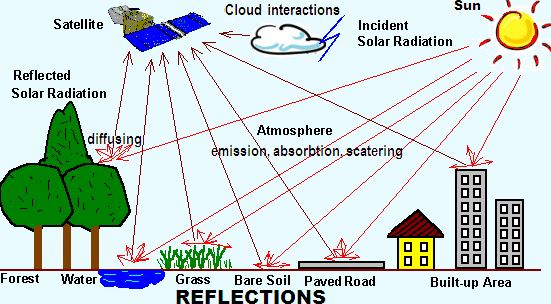
\includegraphics[scale=0.45]{imgs/remote_sensing.JPG}\
		\centering
	\end{figure}
	
\end{frame}

%---------------------------------------------------------

\begin{frame}{La Teledetección de nuestro lado}
	\textbf{Limitaciones:}
	\begin{itemize}
		\item <1-> Diferenciar un cultivo de otro es complicado
		\begin{itemize}
			\item Elevación
			\item Propiedad del suelo
			\item Temperatura
			\item Humedad
			\item Fertilización
			\item Sistema de irrigación
			\item Fecha de plantación
			\item Técnicas y Operación del cultivo
		\end{itemize}
		\item <2-> Similitud en reflectancia y variaciones espaciales, espectrales relacionados a la fenología del cultivo
		\item <3-> Método no fácil de interpretar y operar 
	\end{itemize}
\end{frame}

%---------------------------------------------------------

\begin{frame}
	\frametitle{Artículo Científico}
	
	\begin{figure}
		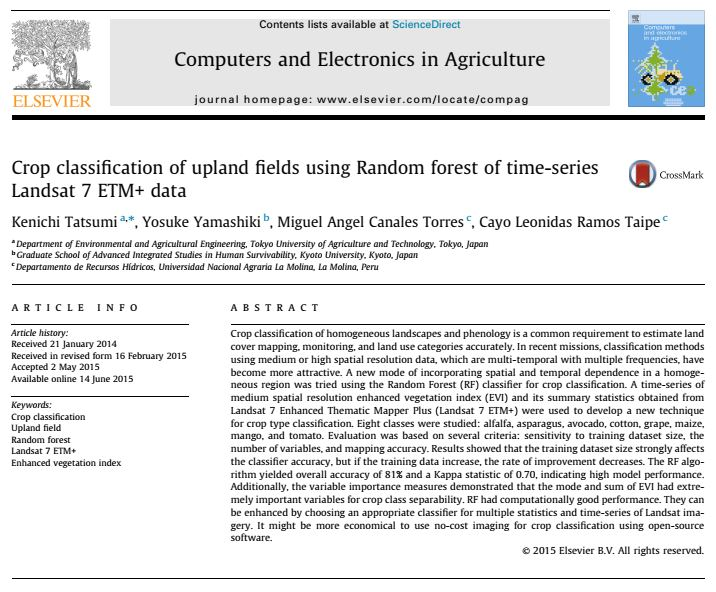
\includegraphics[scale=0.4]{imgs/paper.JPG}\\
		\footnotesize{http://dx.doi.org/10.1016/j.compag.2015.05.001}
		\centering
	\end{figure}
\end{frame}
\section{Objetivos}

%---------------------------------------------------------

\begin{frame}
	\frametitle{Objetivos}
	\textbf{Objetivo Principal}
	\begin{itemize}
		\item Evaluar el desempeño del  \textit{método de clasificación Random Forest} para clasificar ocho tipos de cultivos en terreno homogéneo de aproximadamente 23,000 has usando variables predictoras obtenidas únicamente del producto Landsat 7 ETM+ en el valle de Chincha, Ica.
	\end{itemize}
	
	\textbf{Objetivo Secundario}
	\begin{itemize} 
		\item Desarrollar una metodología para la clasificación e identificación de cultivos en zonas costeras. 
	\end{itemize}

\end{frame}

%---------------------------------------------------------
\section{Zona de Estudio}

%--------------------------------------------------------

\begin{frame}{Zona de estudio}
	\begin{minipage}{0.5\textwidth}
		Datos Generales:
		\begin{itemize}
			\item Ubicación: 13°S, 75.1°W
			\item Superficie a evaluar: 23,000 Has (Aprox.)
			\item Rango de Elevaciones: 0-350 m
			\item Terreno homogéneo
			\item Clima desértico
			\item Tipo de cultivos: Alfalfa, Algodón, Espárrago, Mango, Maíz, Palta, Uva, Tomate.
		\end{itemize}
	\end{minipage} \hfill
	\begin{minipage}{0.45\textwidth}
		\begin{figure}
			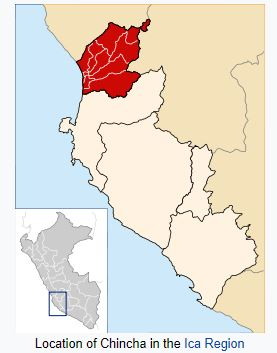
\includegraphics[scale=0.5]{imgs/chincha_ubic.JPG}
			\caption{Fuente: Wikipedia}
		\end{figure}
		
	\end{minipage}
\end{frame}

%---------------------------------------------------------

\begin{frame}{Zona de estudio}
	\begin{figure}[H]
		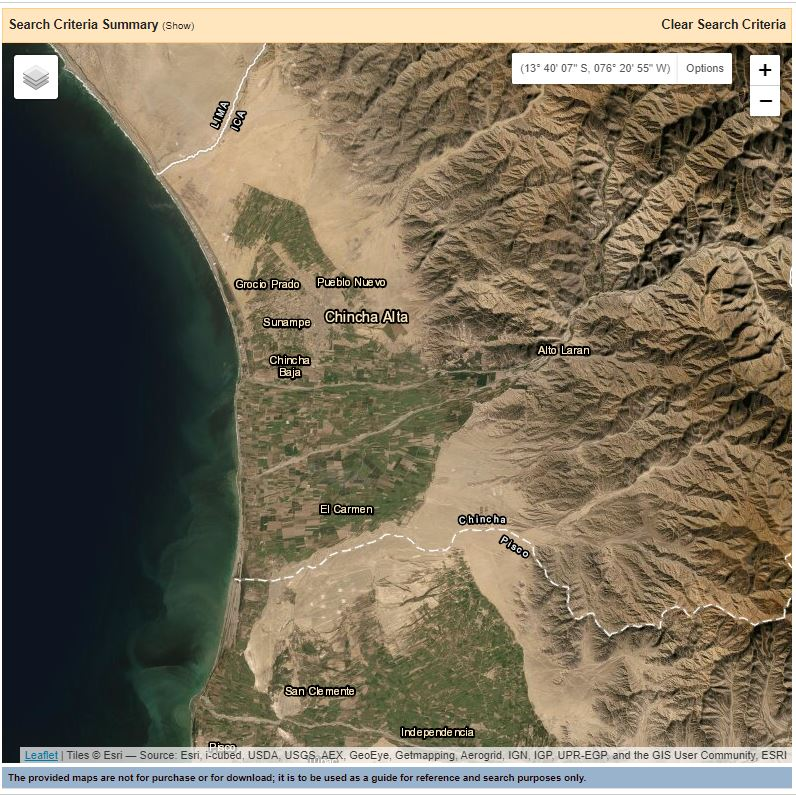
\includegraphics[width=0.75\textheight]{imgs/visualizacion_4.JPG}
		\caption{USGS Earthexplorer}
	\end{figure}
\end{frame}

\section{Metodología}

\begin{frame}
	\frametitle{Metodología}
	La metodología realizada fue la siguiente:
	
	\begin{enumerate}
		\item Preprocesamiento de imágenes satelitales 
		\item Aplicación del Índice EVI 
		\item Método Random Forest
		\item Validación de resultados
	\end{enumerate}
\end{frame}

%---------------------------------------------------------
{
	\setbeamertemplate{background canvas}
	{
		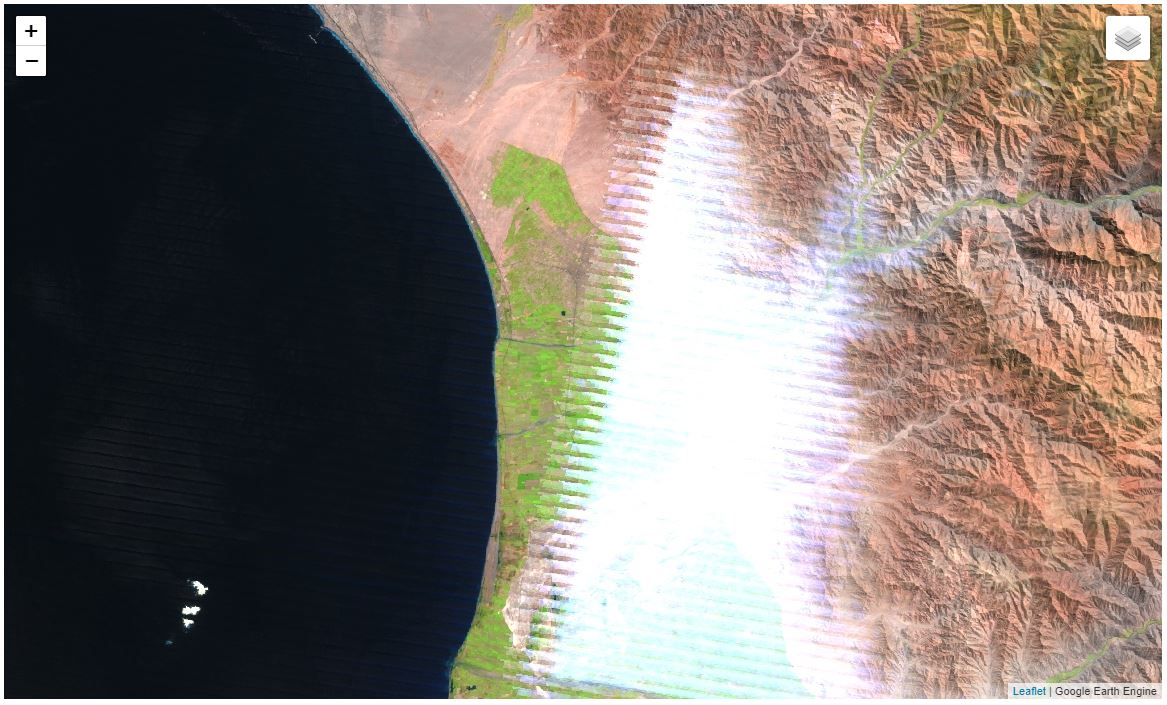
\includegraphics[width=\paperwidth,height=\paperheight]{imgs/pre_process_1.JPG}
	}
	\begin{frame}{Landsat 7 ETM sin tratar}
	\end{frame}
}
%---------------------------------------------------------
{
	\setbeamertemplate{background canvas}
	{
		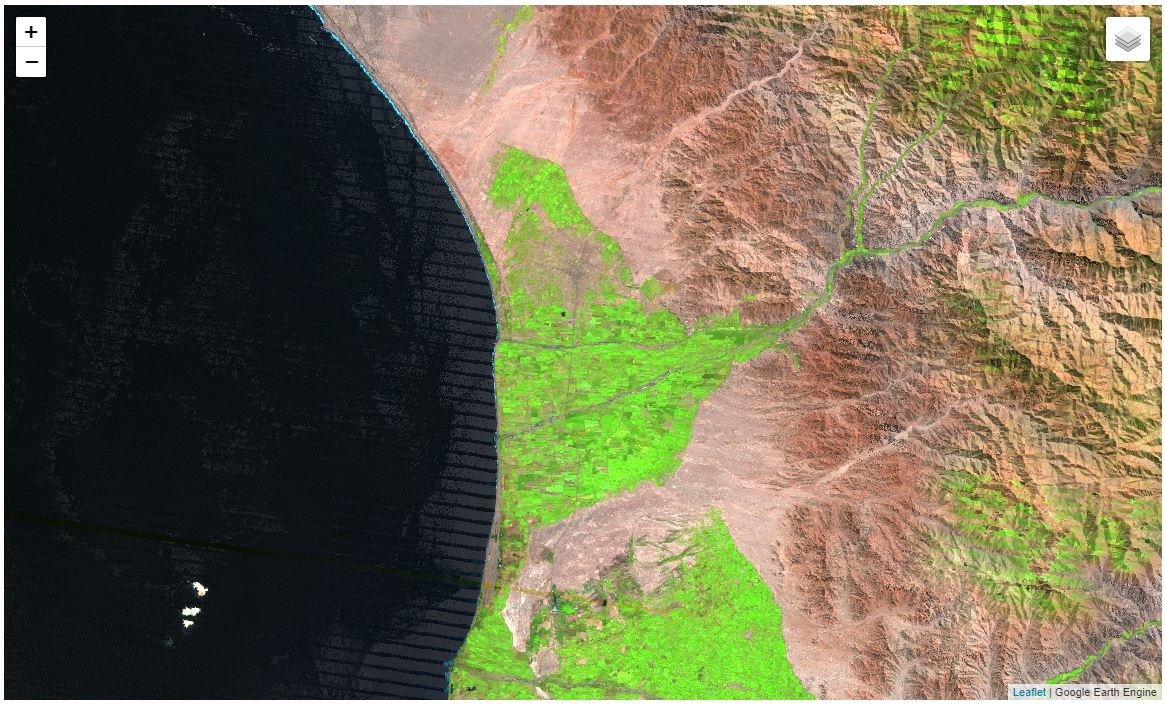
\includegraphics[width=\paperwidth,height=\paperheight]{imgs/pre_process_2.JPG}
	}
	\begin{frame}{Landsat 7 ETM tratada}
	\end{frame}
}
%--------------------------------------------------------
{
	\setbeamertemplate{background canvas}
	{
		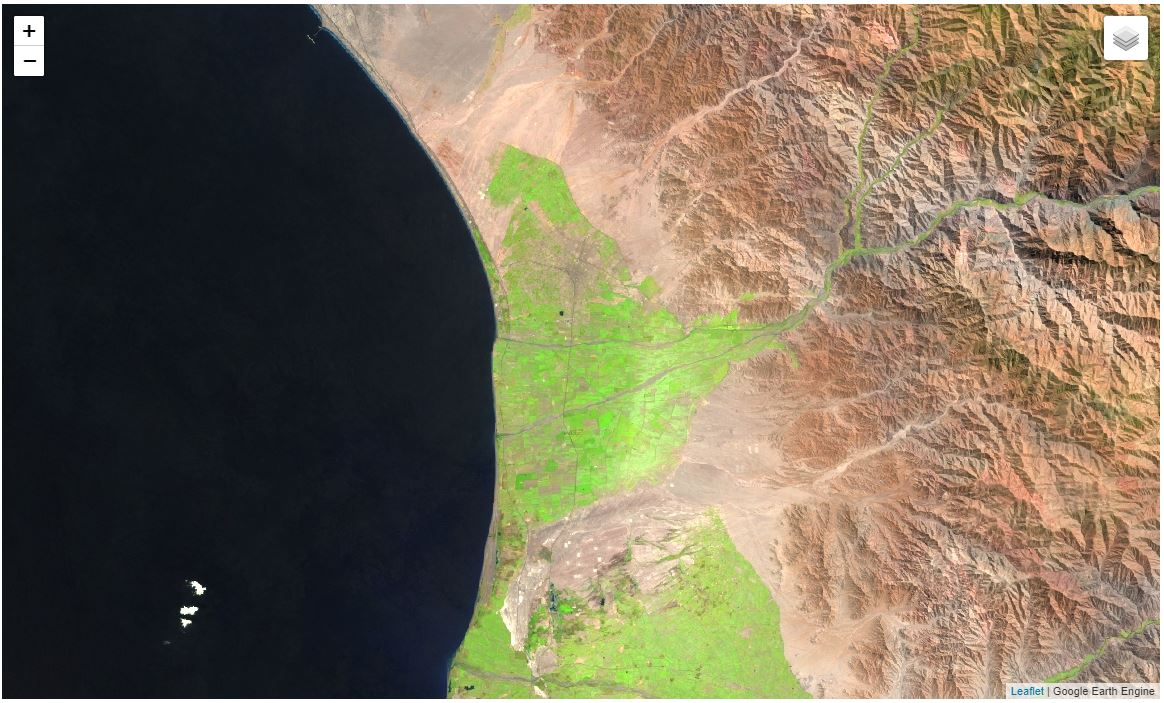
\includegraphics[width=\paperwidth,height=\paperheight]{imgs/pre_process_3.JPG}
	}
	\begin{frame}{Evaluando otros productos disponibles - Landsat 8}
	\end{frame}
}
%--------------------------------------------------------
\begin{frame}{Indice de Vegetación Mejorado - EVI}
	\begin{figure}
		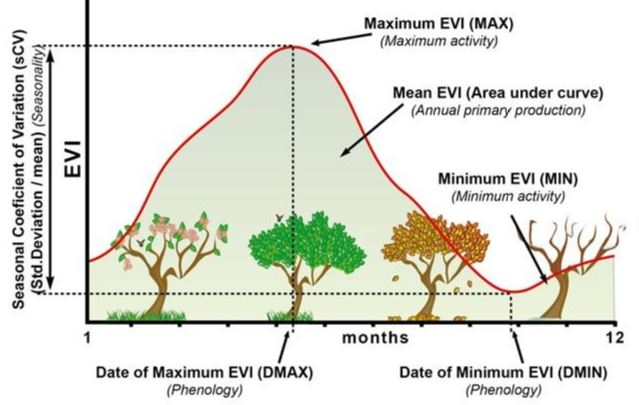
\includegraphics[scale=0.55]{imgs/EVI.JPG}
		\caption{EVI}
	\end{figure}
\end{frame}
%--------------------------------------------------------

\begin{frame}{Aplicación del EVI}
	\begin{figure}
		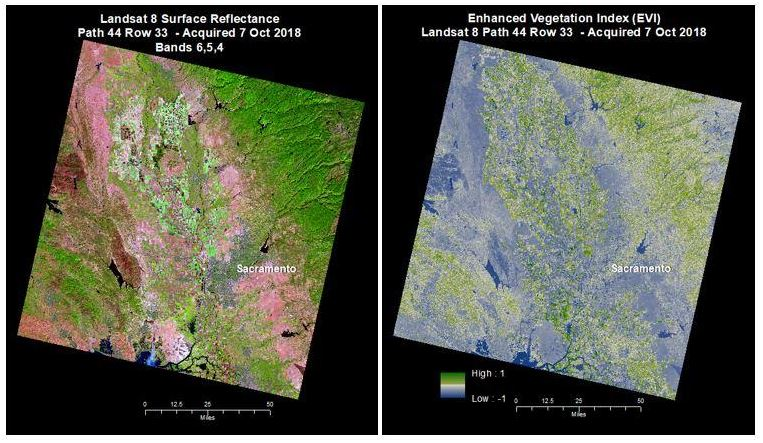
\includegraphics[scale=0.5]{imgs/EVI_result.JPG}
		\caption{Fuente: USGS}
	\end{figure}
\end{frame}
%--------------------------------------------------------

\begin{frame}{Método Random Forest}
	\begin{figure}
		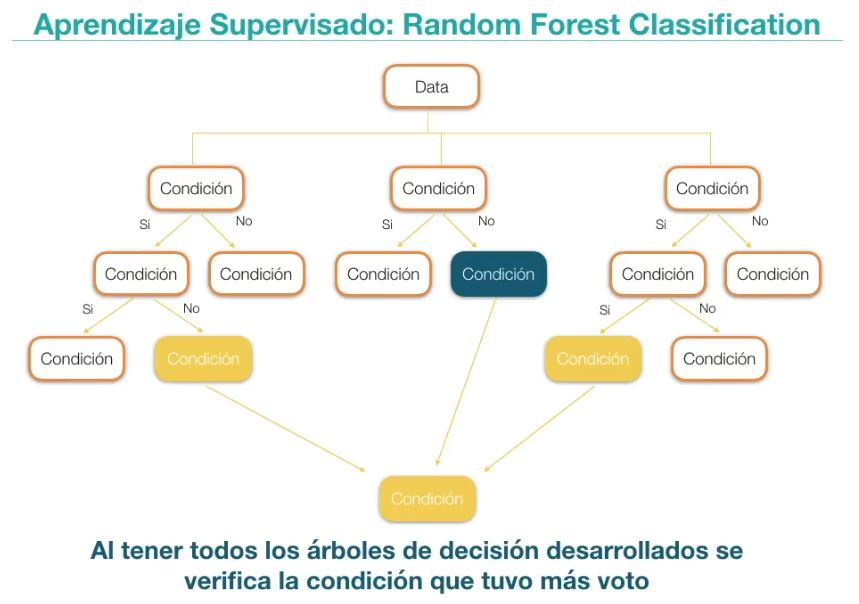
\includegraphics[scale=0.4]{imgs/random_forest.JPG}\\
		\caption{Curso de Introducción a Machine Learning - Ligdi Gonzalez - Youtube}
	\end{figure}
\end{frame}

%--------------------------------------------------------

\begin{frame}{Método Random Forest}
	\begin{figure}
		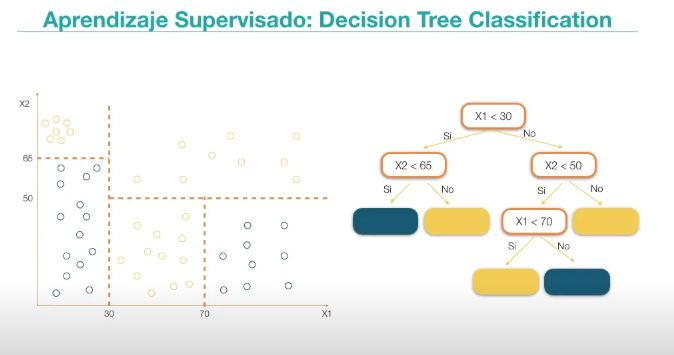
\includegraphics[scale=0.6]{imgs/random_forest_1.JPG}\\
		\caption{Curso de Introducción a Machine Learning - Ligdi Gonzalez - Youtube}
	\end{figure}
\end{frame}
\section{Resultados}

%---------------------------------------------------------

\begin{frame}{Validación de resultados}

\begin{figure}
	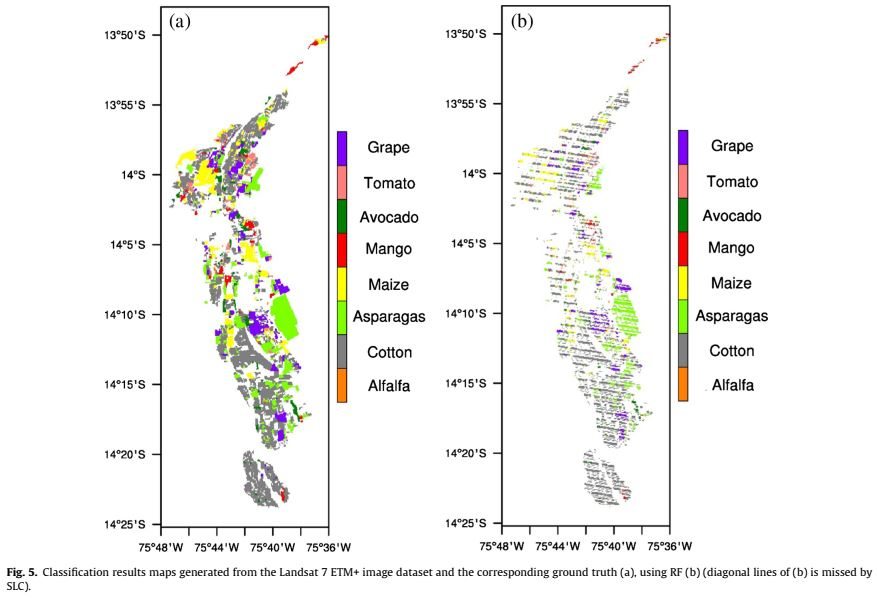
\includegraphics[scale=0.4]{imgs/resultado_paper.JPG}\\
	\centering
\end{figure}

\end{frame}

%---------------------------------------------------------
\section{Conclusiones}

\begin{frame}{Conclusiones}
	Debe responder estas preguntas:
	\begin{itemize}
		\item ¿Es efectivo aplicar Random Forest para clasificar e identificar cultivos?
		\item ¿Como se midió su efectividad?
		\item ¿Dónde no es posible aplicar este método de clasificación?
		
	\end{itemize}
\end{frame}



%---------------------------------------------------------

\begin{frame}{}
	\centering \Huge
	\emph{¡Gracias CIDRHI!}
\end{frame}

\end{document}